\documentclass[11pt,a4paper]{article}
\usepackage[margin=2.2cm]{geometry}
\usepackage{fontspec}
\setmainfont{Garuda}[Scale=1.05]
\usepackage{amsmath,amssymb}
\usepackage{tikz}
\usetikzlibrary{arrows.meta,calc}
\usepackage{parskip}
\setlength{\parindent}{0pt}
\linespread{1.2}
\begin{document}
\begin{center}\Large\bfseries โจทย์ฟิสิกส์ ข้อ 51--60\end{center}
\bigskip
\par\noindent\textbf{51.}\quad (IJSO รอบที่ 2 2553) พนักงานขับรถไฟคนหนึ่งหลับในขณะที่กำลังขับรถไฟขบวนหนึ่งด้วยอัตราเร็ว $v$ อยู่บนทางตรง เขาสะดุ้งตื่นขึ้นมาเมื่อได้ยินเสียงดังเอะอะ และพบว่ามีรถไฟอีกขบวนหนึ่งอยู่ข้างหน้าที่ระยะห่าง $d$ และกำลังแล่นไปทางเดียวกันด้วยอัตราเร็ว $u$ ซึ่งช้ากว่าขบวนของเขา พนักงานขับรถไฟตัดสินใจดึงห้ามล้อทันที ทำให้รถไฟด่วนมีความหน่วงคงตัวขนาดเท่ากับ $a$ จงหาว่า $d$ ต้องมีค่าเป็นอย่างไร จึงจะไม่เกิดการชนท้ายขึ้น\par\medskip

\par\noindent\textbf{52.}\quad (สอวน ม.4 2549) รถไฟขบวนหนึ่งกำลังแล่นด้วยอัตราเร็ว $v_A$ ไปตามรางตรง ทันใดนั้นพนักงานขับรถก็สังเกตเห็นรถไฟอีกขบวนหนึ่งที่ระยะห่าง $d$ กำลังแล่นอยู่ข้างหน้าไปในทิศทางเดียวกันด้วยอัตราเร็ว $v_B$ เขาจึงดึงห้ามล้อทันที ถ้ารถไฟแล่นต่อด้วยความหน่วงคงตัว และรถไฟขบวนหน้าแล่นด้วยความเร็วเท่าเดิมไปเรื่อยๆ จงหาความหน่วงที่น้อยที่สุดที่จะทำให้หลีกเลี่ยงการชนกับรถไฟขบวนหน้าได้พอดี\par\medskip

\par\noindent\textbf{53.}\quad (สอวน ม.4 2550) รถไฟ $A$ และ $B$ สองขบวนแล่นบนรางตรงเดียวกันมาในทิศทางตรงกันข้าม พนักงานขับรถทั้งสองต่างเห็นรถไฟอีกขบวนหนึ่งอยู่ข้างหน้า จึงดึงห้ามล้อพร้อมกันเมื่อรถไฟทั้งสองอยู่ห่างกัน $D$ และมีอัตราเร็วตอนนั้น $u_A$ และ $u_B$ สมมติว่ารถไฟทั้งสองขบวนเคลื่อนที่ช้าลงด้วยความหน่วงคงตัว และรถไฟหยุดพร้อมกันที่ระยะห่าง $d$

\par\smallskip 53.1\quad จงหาอัตราส่วนขนาดความหน่วงของรถไฟ $B$ ต่อขนาดความหน่วงของรถไฟ $A$

\par\smallskip 53.2\quad จงหาขนาดความหน่วงของรถไฟ $A$\par\medskip

\par\noindent\textbf{54.}\quad (สอวน ม.4 2546) ปล่อย $m_1$ จากหยุดนิ่งที่จุด $A$ พร้อมกันกับที่ดีด $m_2$ ขึ้นไปในแนวดิ่งจากจุด $B$ ใต้จุด $A$ ด้วยความเร็วต้น $u$ มวลทั้งสองจะชนกันเมื่อ $m_1$ ตกลงมาเป็นระยะทางเท่าไร กำหนดให้ระยะ $AB$ เท่ากับ $h$
\begin{center}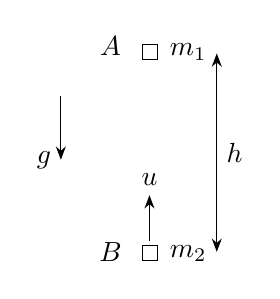
\begin{tikzpicture}[>=Stealth,scale=.9]
\node at (0,2.9) {$A$};\draw (0.45,2.72) rectangle (.66,2.93);\node[right] at (.7,2.82) {$m_1$};
\node at (0,0) {$B$};\draw (.45,-.12) rectangle (.66,.09);\node[right] at (.7,-.02) {$m_2$};
\draw[<->] (1.5,0)--node[right]{$h$}(1.5,2.8);\draw[->] (.55,.16)--(.55,.8) node[above]{$u$};\draw[->] (-.7,2.2)--(-.7,1.3) node[left]{$g$};
\end{tikzpicture}\end{center}\par\medskip

\par\noindent\textbf{55.}\quad (สอวน ม.4 2549) โยนวัตถุ $A$ ขึ้นในแนวดิ่งด้วยอัตราเร็ว $u$ และที่เวลา $u/g$ ต่อมาก็โยนวัตถุ $B$ ตามขึ้นไปด้วยอัตราเร็ว $u$ เท่ากัน ถ้าวัตถุทั้งสองชนกันเหนือพื้น จงหาความสูงของตำแหน่งที่วัตถุทั้งสองชนกัน ในที่นี้ $g$ คือขนาดความเร่งสนามโน้มถ่วงโลกที่บริเวณนั้น\par\medskip

\par\noindent\textbf{56.}\quad (สอวน ม.4 2550) ปล่อยวัตถุ $A$ จากหยุดนิ่งลงมาจากที่สูง $H$ ที่เวลา $\sqrt{\dfrac{H}{2g}}$ หลังจากนั้นก็ปาวัตถุ $B$ ตามลงมา จงหาว่าจะต้องปา $B$ ด้วยอัตราเร็วเท่าใด จึงจะไล่ทัน $A$ ที่พื้นพอดี\par\medskip

\par\noindent\textbf{57.}\quad (สอวน ม.4 2554) ปล่อยลูกปิงปองให้ตกในแนวดิ่งกระทบพื้นราบครั้งแรกด้วยความเร็วต้นมีขนาด $v_0$ ลูกปิงปองกระดอนขึ้นด้วยความเร็ว $v_1=e v_0$ [$e$ มีค่าน้อยกว่า 1] ลูกปิงปองจะกระทบพื้นครั้งที่สองหลังครั้งแรกเป็นเวลานานเท่าไร ตอบในรูป $v_0$, $e$ และ $g$
\begin{center}\begin{tikzpicture}[>=Stealth,scale=.9]
\draw[dashed] (-1.5,0)--(2,0);\foreach \x in {-1.2,-.9,-.6,-.3,0,.3,.6,.9,1.2,1.5}{\draw (\x,0)--++(-.13,-.12);}
\draw (0,2.4) circle (.12);\draw[dashed] (0,2.25)--(0,.15);\draw (0,.12) circle (.12);\draw[->] (0,-.1)--(0,-.8) node[below]{$v_0$};
\draw (1,.12) circle (.12);\draw[->] (1,.3)--(1,1.25) node[above]{$v_1=e v_0$};\node[right] at (1.4,.12) {พื้นแข็ง};
\draw[->] (-1.4,1.6)--(-1.4,.8) node[left]{$g$};
\end{tikzpicture}\end{center}\par\medskip

\par\noindent\textbf{58.}\quad (สอวน ม.4 2556) ลูกบอลลูกหนึ่งกระดอนในแนวดิ่งจากพื้นแข็งแบบที่อัตราส่วน
\[\frac{\text{ขนาดความเร็วหลังกระดอนทันที}}{\text{ขนาดความเร็วก่อนกระทบพื้น}}\]
เท่ากับ $e$ คงที่ $<1$.

ปล่อยลูกบอลจากความสูง $h_0$ มันกระดอนครั้งแรกขึ้นไปได้สูง $h_1$ ครั้งที่สองขึ้นไปได้สูง $h_2$, ฯลฯ จงหาความสูงที่มันขึ้นไปได้หลังครั้งที่ $n$ ตอบในรูปของ $e,n,h_0$
\begin{center}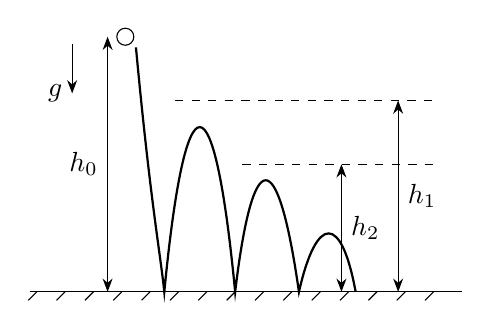
\begin{tikzpicture}[>=Stealth,scale=.9]
\draw (-.5,0)--(5.6,0);\foreach \x in {-.4,0,...,5.5}{\draw (\x,0)--++(-.12,-.12);}
\draw[->] (.1,3.5)--(.1,2.8) node[left]{$g$};\draw (.85,3.6) circle (.12);
\draw[thick] (1,3.45) .. controls (1.2,1.3) and (1.35,.5) .. (1.4,0) .. controls (1.7,3.1) and (2.1,3.1) .. (2.4,0) .. controls (2.65,2.1) and (3,2.1) .. (3.3,0) .. controls (3.55,1.1) and (3.9,1.1) .. (4.1,0);
\draw[dashed] (1.55,2.7)--(5.2,2.7);\draw[dashed] (2.5,1.8)--(5.2,1.8);
\draw[<->] (.6,0)--node[left]{$h_0$}(.6,3.6);\draw[<->] (4.7,0)--node[right]{$h_1$}(4.7,2.7);\draw[<->] (3.9,0)--node[right]{$h_2$}(3.9,1.8);
\end{tikzpicture}\end{center}\par\medskip

\par\noindent\textbf{59.}\quad (สอวน ม.5 2554, 2556; สสวท รอบที่ 1 2548) ลูกบอลลูกหนึ่งเมื่อเคลื่อนที่เข้ากระทบตั้งฉากกับพื้นแข็งด้วยความเร็วขนาด $v_0$ จะกระดอนกลับด้วยความเร็ว $v_1=e v_0$ ซึ่ง $e$ มีค่าน้อยกว่า 1.

ถ้าปล่อยลูกบอลนี้จากความสูง $h$ ให้ตกด้วยความเร่ง เนื่องจากแรงโน้มถ่วง $g$ เข้ากระทบพื้นระดับที่แข็ง มันก็จะกระดอนขึ้นลงๆ มันจะกระดอนอยู่เป็นเวลาเท่าใด

ตอบในเทอมของ $e,g$ และ $h$.\par\medskip

\par\noindent\textbf{60.}\quad (IJSO รอบที่ 1 2557) แรง $A$ และแรง $B$ กระทำต่อวัตถุที่ตำแหน่ง $X$ ด้วยขนาดและทิศทางดังแสดงด้วยลูกศร ดังรูป ความเร่งของวัตถุมีทิศใกล้เคียงกับข้อใดมากที่สุด
\begin{center}\begin{tikzpicture}[>=Stealth,scale=1]
\coordinate (X) at (0,0);\draw[->,thick] (X)--(-.9,1.15) node[left]{$A$};\draw[->,thick] (X)--(1.55,1.35) node[right]{$B$};\node[below] at (X) {$X$};
\begin{scope}[yshift=-1.5cm]\foreach \i/\dx/\dy in {1/-1/-.35,2/1/.4,3/-.3/-1,4/.35/1}{\pgfmathsetmacro{\xx}{(\i-1)*2.4-3.5}\node at (\xx-.5,0) {\i.};\draw[->,thick] (\xx,0)--++(\dx,\dy);}\end{scope}
\end{tikzpicture}\end{center}\par\medskip

\end{document}
